Un diseñador gráfico está creando un logotipo a partir de una figura geométrica compuesta. Parte de un cuadrado de lado 6 cm y agrega regiones curvas en algunos de sus lados para darle un diseño más dinámico. Explique con sus palabras el procedimiento necesario para resolver el problema.

\begin{center}
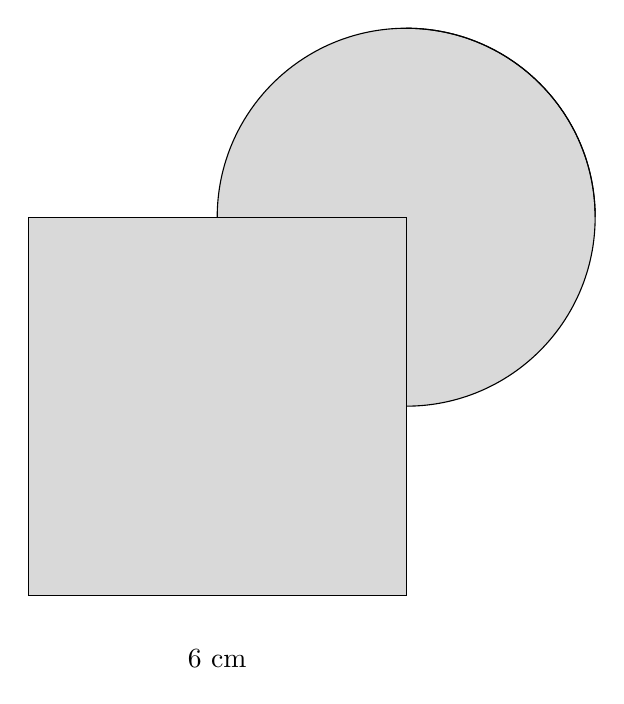
\begin{tikzpicture}[scale=0.8]

% Cuadrado
\fill[gray!30] (0,0) rectangle (6,6);

% Semicírculos (3 lados)
\fill[gray!30] (3,6) arc[start angle=180,end angle=0,radius=3];
\fill[gray!30] (6,3) arc[start angle=-90,end angle=90,radius=3];

% Bordes
\draw (0,0) rectangle (6,6);
\draw (3,6) arc[start angle=180,end angle=0,radius=3];
\draw (6,3) arc[start angle=-90,end angle=90,radius=3];

% Medida
\node at (3,-1) {6 cm};

\end{tikzpicture}
\end{center}

¿Cuál de las siguientes expresiones representa el área total de la figura?

\begin{multicols}{2}
\begin{enumerate}[label=\alph*), leftmargin=*]
\item $36 + 6\pi$
\item $36 + 9\pi$
\item $36 + 18\pi$
\item $36 + \frac{3}{2}\pi(3^2)$
\end{enumerate}
\end{multicols}